% >>>>>>>>>>>>>>>>>>>>>>>>>>>>>>>>>>>>>>>>>>>>
% Dimensions
% <<<<<<<<<<<<<<<<<<<<<<<<<<<<<<<<<<<<<<<<<<<<
\newdimen\bottomHeight%
\bottomHeight=.15\textheight%
% The following empty line is intentional!

% >>>>>>>>>>>>>>>>>>>>>>>>>>>>>>>>>>>>>>>
% Seperation Line
% <<<<<<<<<<<<<<<<<<<<<<<<<<<<<<<<<<<<<<<
%\vfill%
\begin{minipage}[t][\seplineHeight][b]{\textwidth}%
%\fbox{%
\vbox to \seplineHeight{%
\vfill%
\begin{center}%
\textcolor{sky}{%
\rule{\textwidth}{.2mm}}%
\end{center}%
\vfill%
}%
%}%
\end{minipage}%
\noindent%

\begin{minipage}[b][\midHeight][t]{.34\textwidth}%
{\color{BaseDarkColor}\usebeamerfont{block title} Key Insight from \cref{eq:estimate}:}
%
\begin{block}{}
\centering%
\textit{%
\enquote{Ratio convergence rates for the distance function imply convergence rates for AMLEs.}}
\end{block}
%
In \cite{bungert2021uniform} we prove:
\abovedisplayskip=0pt%
\belowdisplayskip=0pt%
\begin{align*}
\abs{x-y} \leq 
\sigma_\eta d_n(x,y)
\leq 
\left(1 + C \frac{\gres_n}{\gscale_n}\right) 
\abs{x-y} + \tau_\eta \, \gscale_n,
\end{align*}
where
$\sigma_\eta := \sup_{t>0}\eta(t)t$ and $\tau_\eta := \sup_{t>0}\sigma_\eta\eta(t)^{-1}-t.$
%
\vspace{.2em}

\fbox{%
\begin{minipage}[b][4cm][c]{\textwidth}%
\textbf{Sparse regime}: If $\gres_n\lesssim\gscale_n\lesssim\gres_n^{\frac{5}{9}}$ the rate is $\left({\gres_n}/{\gscale_n}\right)^{\frac{1}{4}}$.\\
\textbf{Dense regime}: If $\gscale_n\gtrsim\gres_n^{\frac{5}{9}}$ the rate is $\gscale_n^{\frac{1}{5}}$.
\end{minipage}}%
\vspace{.5em}
{\color{BaseDarkColor}\usebeamerfont{block title} \noindent What about $\gscale_n\sim\gres_n$? Percolation!}\\
\small
On a unit intensity Poisson Point Process $X\subset\R^d$ and for $h>0$ let $\Pi_h(x,y)$ be the set of admissible paths and
%
\begin{align*}
T_s := d_{h_s}(0,s e_1) := \inf 
\left\lbrace\sum_{i=1}^{\operatorname{len}(p)-1} \abs{p_{i+1}-p_{i}} \st 
p\in\Pi_{h_s}(0,s e_1)
\right\rbrace.
\end{align*}
%
\alert{Important}: Replace $T_s$ by distance $T_s^\prime$ on an \alert{enriched process} $\mathcal{X}_s$.
\end{minipage}%
%
%
\hfill%
%
%
\begin{minipage}[b][\midHeight][t]{.31\textwidth}%
%
\begin{minipage}{\textwidth}
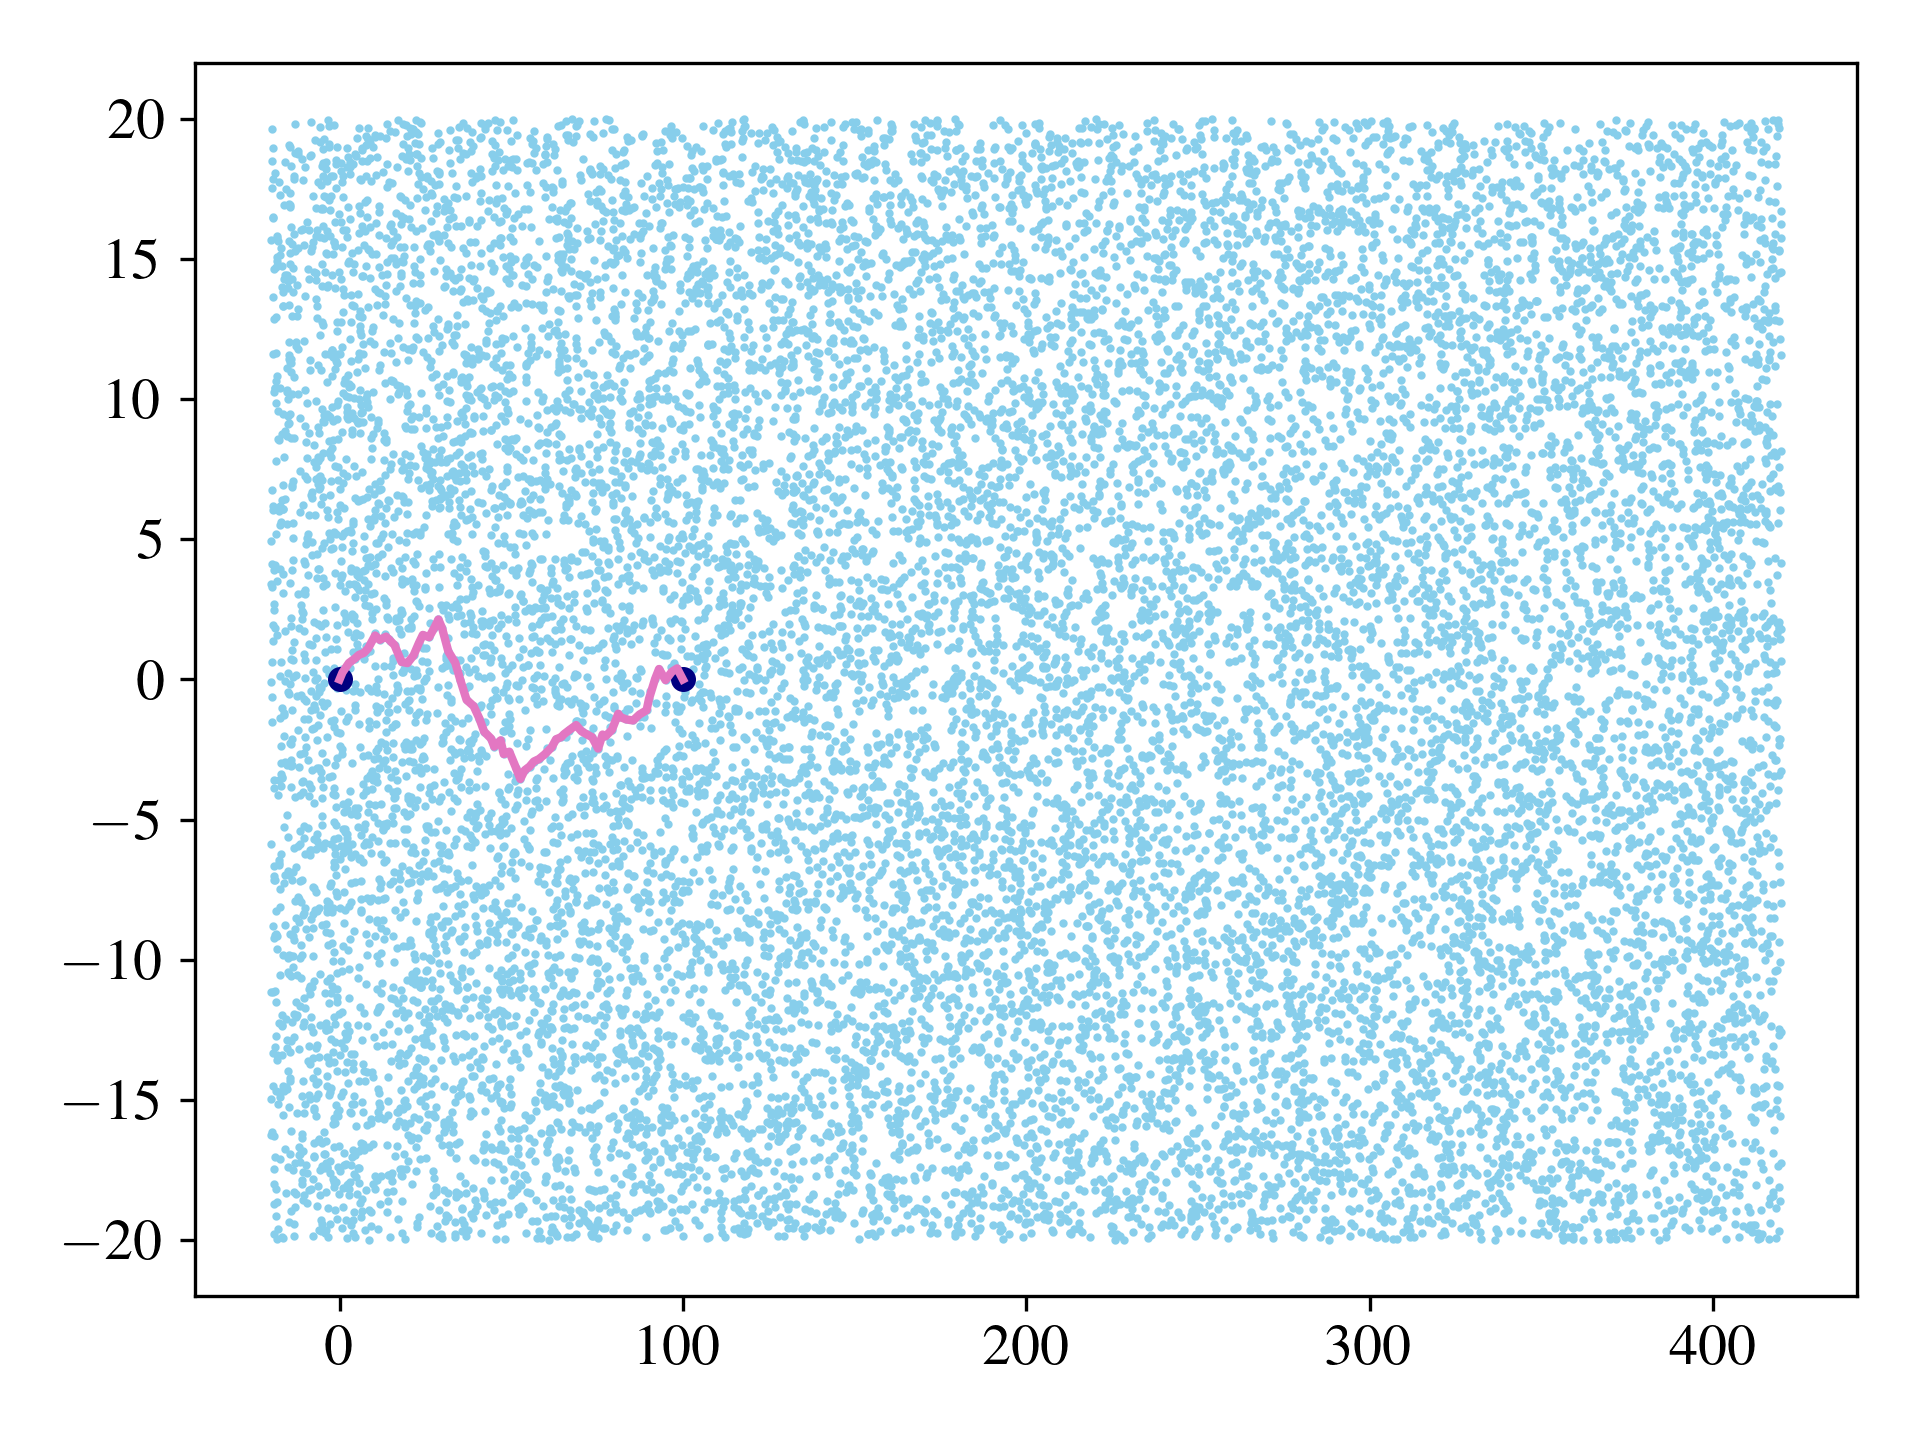
\includegraphics[width=0.3\textwidth]{atelier/path_2d_s-100}
\hfill
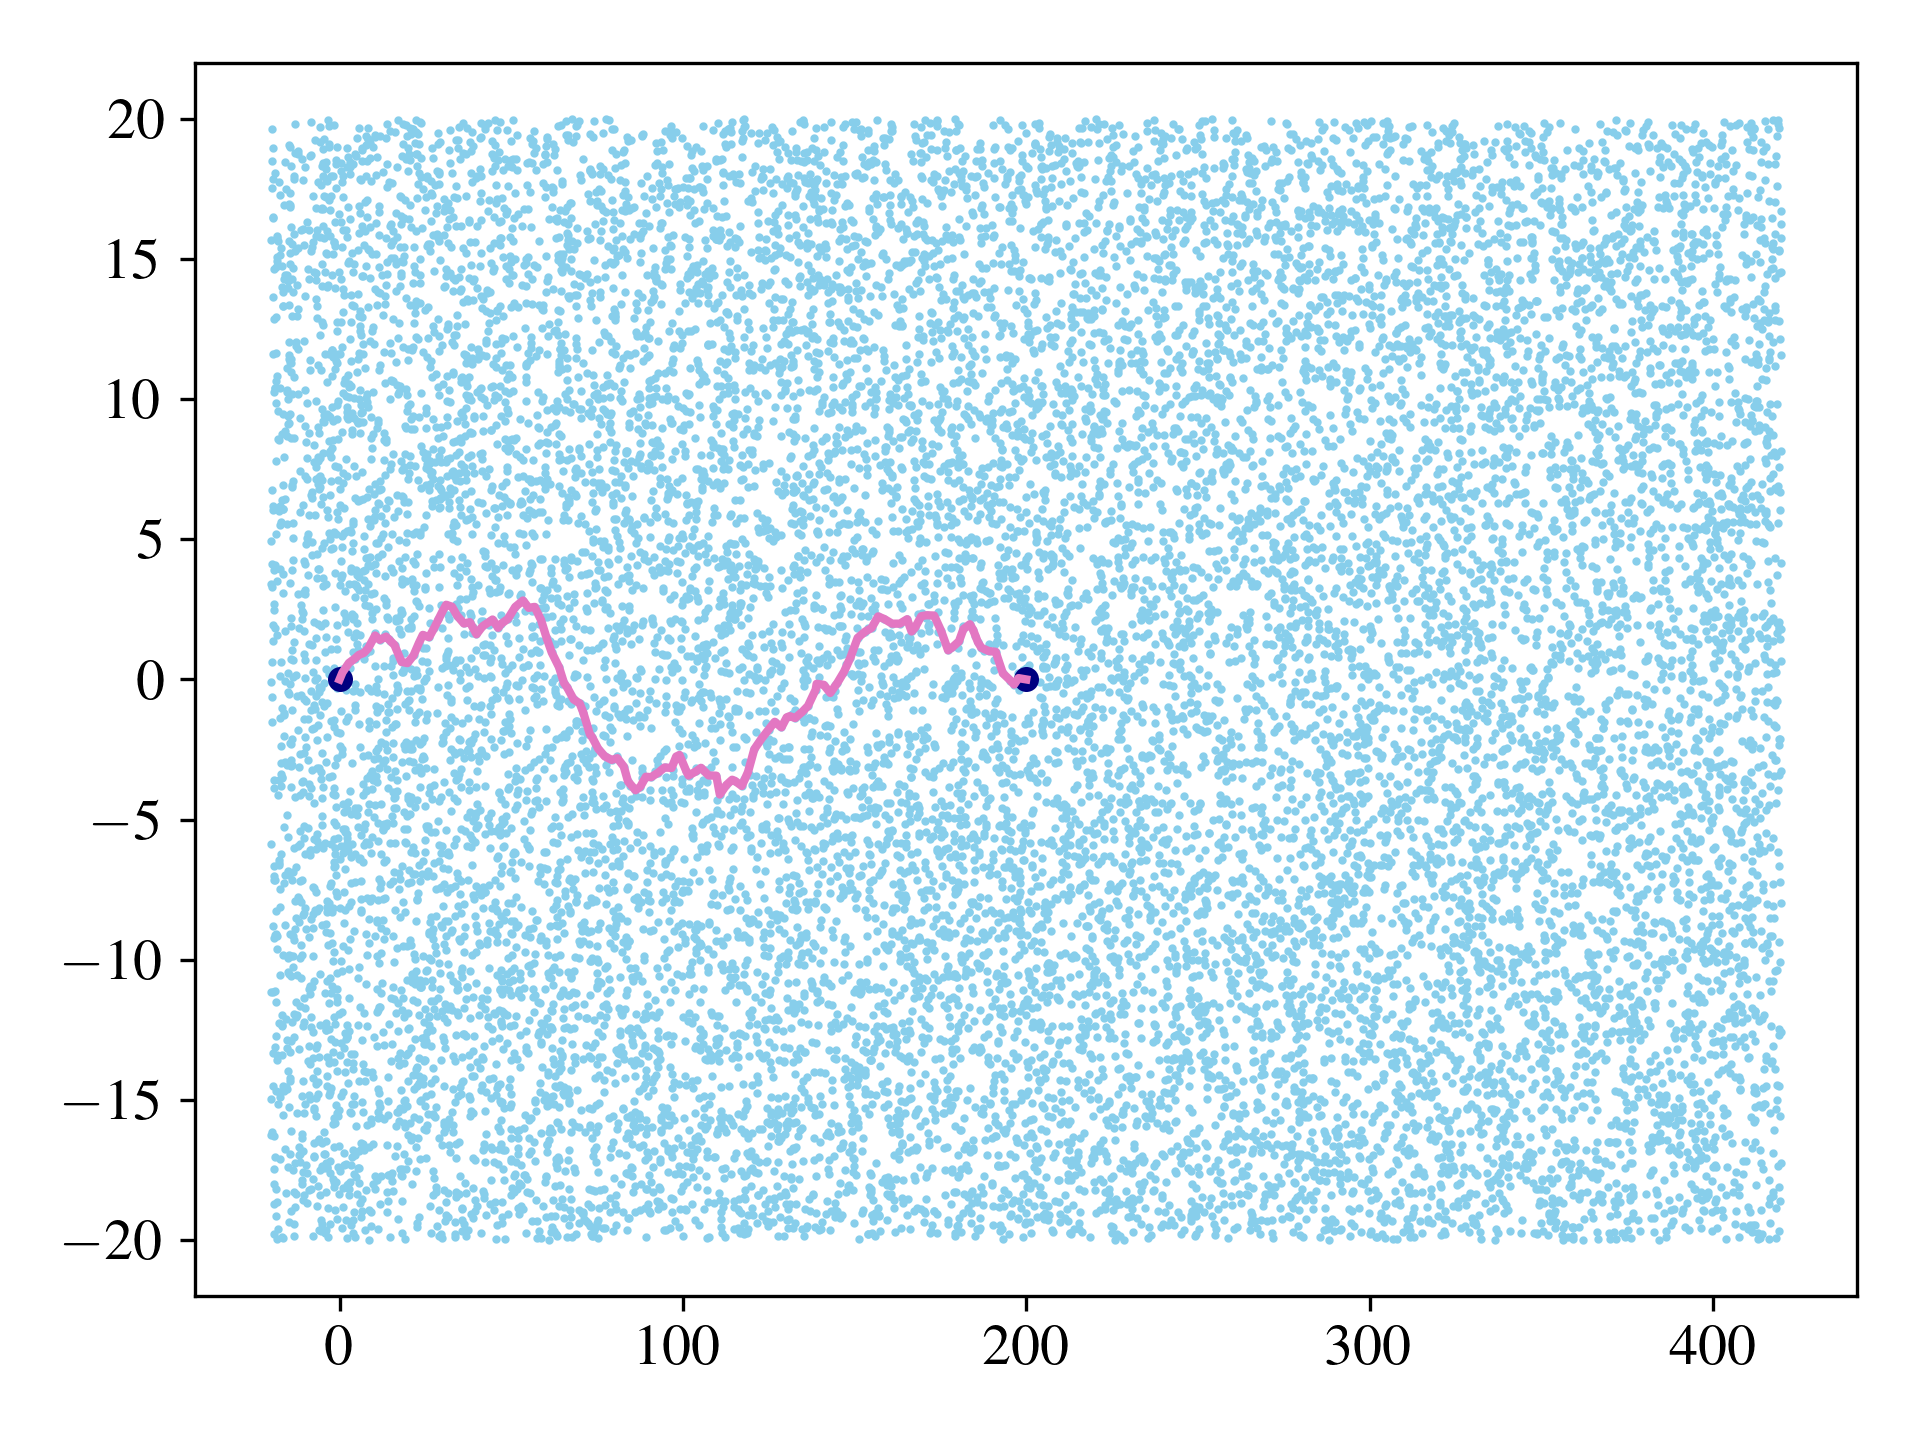
\includegraphics[width=0.3\textwidth]{atelier/path_2d_s-200}
\hfill
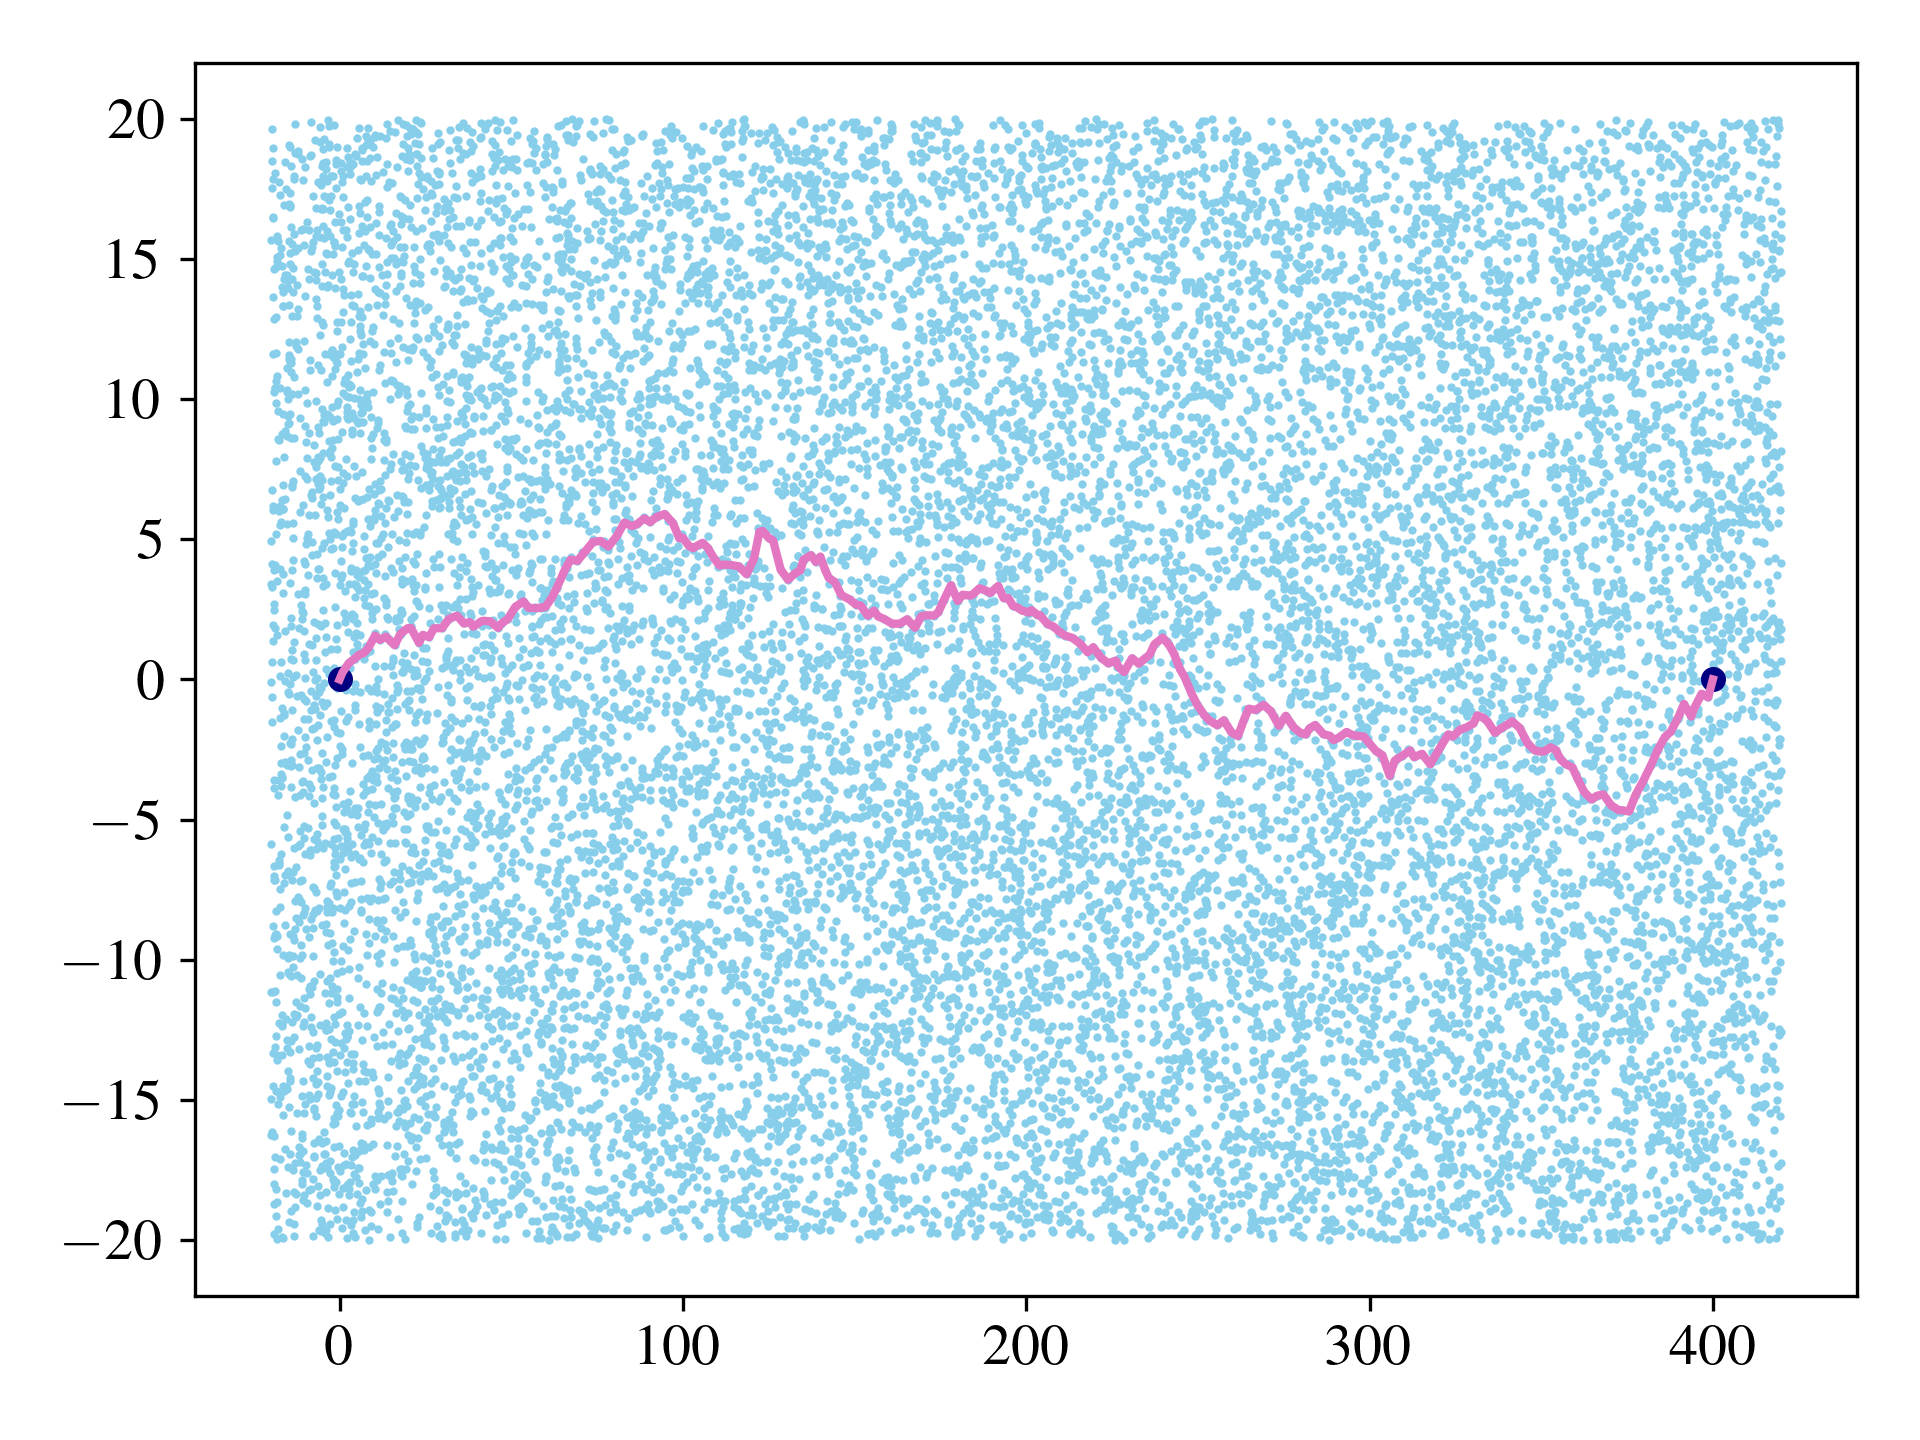
\includegraphics[width=0.3\textwidth]{atelier/path_2d_s-400}
\end{minipage}%

$s\mapsto h_s$ are growing step sizes with $h_s \gtrsim \log(s)^\frac{1}{d}$. 

% For slowly increasing $s\mapsto g(s)$ we have:
\alert{Approximate sub- and superadditivity}:
\begin{alignat*}{2}
    \Exp{T_{s+t}^\prime} &\leq \Exp{T_{s}^\prime} + \Exp{T_{t}^\prime} + g(s+t) \quad &&\text{\color{apple}\ding{52}\nc}
    \\
    \Exp{T_{2s}^\prime} &\geq 2 \Exp{T_s^\prime} - g(s) \quad &&\text{\color{grape}\textbf{???}\nc}
\end{alignat*}
% %
% \textbf{Subadditivity:} $\Exp{T_{s+t}^\prime} \leq \Exp{T_{s}^\prime} + \Exp{T_{t}^\prime} + g(s+t)$ \color{apple}\ding{52}\nc\\
% %
% \textbf{Superadditivity:} $\Exp{T_{2s}^\prime} \geq 2 \Exp{T_s^\prime} - g(s)$ \color{grape}\textbf{???}\nc
For \alert{ratio convergence} it suffices to freeze $h_s$:
\begin{align*}
\Exp{d_{h_s,\mathcal{X}_s}(0,2se_1)} \geq 2 \Exp{d_{h_s,\mathcal{X}_s}(0,s)} - g(s).
\end{align*}
%
With \alert{concentration of measure} we get \cite{bungert2022ratio}
%
\begin{block}{}
\begin{align*}
\abs{\frac{\Exp{d_{h_s,\mathcal{X}_s}(0,se_1)}}{\Exp{d_{h_s,\mathcal{X}_s}(0,2se_1)}} - \frac{1}{2}}
&\lesssim
\sqrt{\frac{\log(s)^{2/d}}{h_s}}\frac{\log(s)}{\sqrt{s}}\\
%
\Rightarrow \max_{\domain_n}\abs{\vec u_n - u} 
&\lesssim 
\log(n)^{2/9}\gres_n^{1/9}.
\end{align*}
\end{block}
\end{minipage}%
%
\hfill%
%
\begin{minipage}[b][\midHeight][t]{.31\textwidth}%
{\color{BaseDarkColor}\usebeamerfont{block title} Numerical Examples}\\
\begin{minipage}{.5\textwidth}%
\small%
Infinity harmonic function $u(x_1,x_2)=\abs{x_1}^{4/3}-\abs{x_2}^{4/3}$ on $\domain:=\{\abs{x_1}^{2/3}+\abs{x_2}^{2/3}\leq 1\}.$
\end{minipage}%
\begin{minipage}{.5\textwidth}%
\centering
{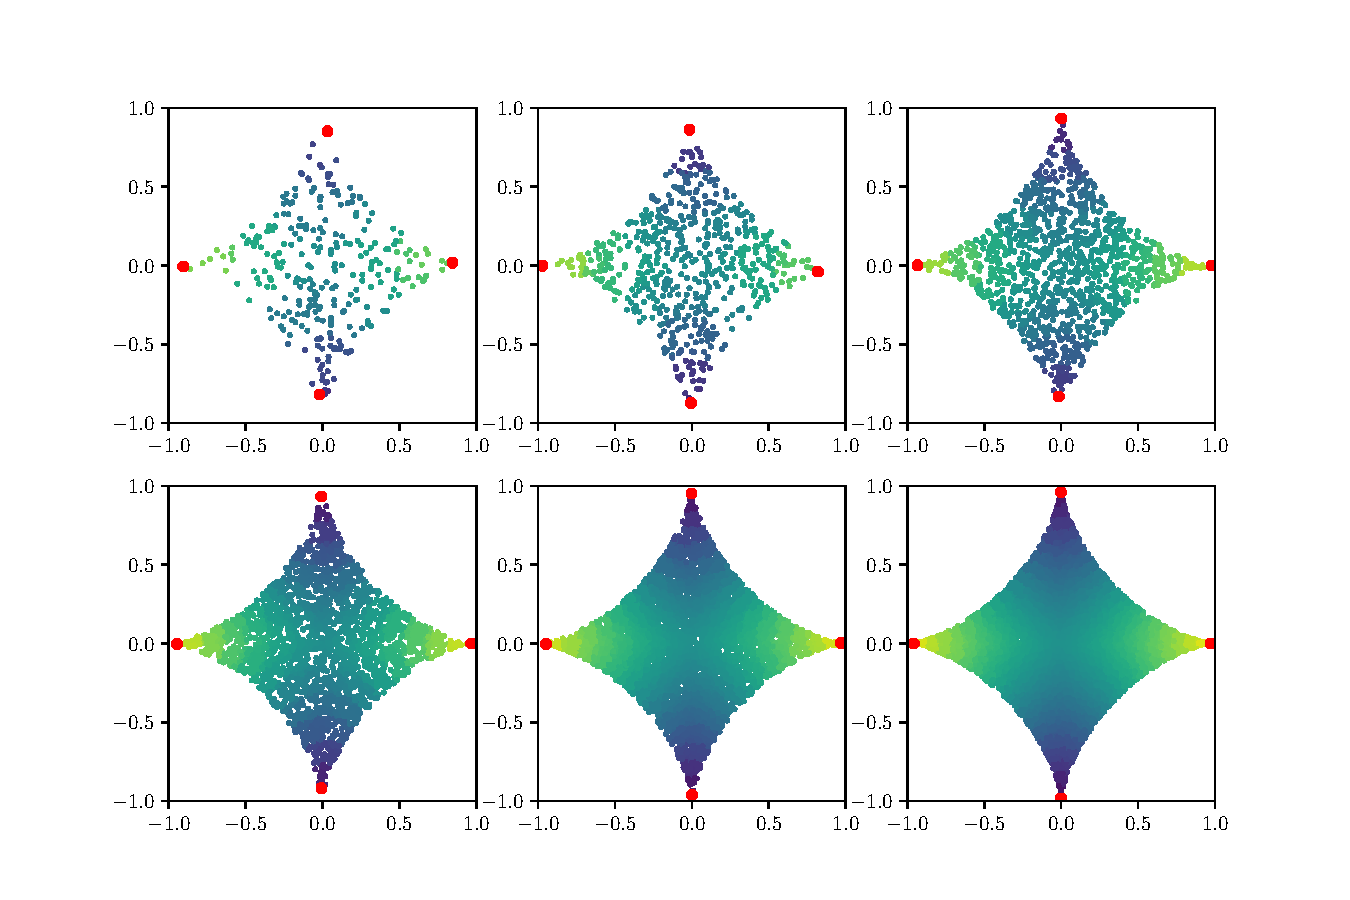
\includegraphics[width=0.8\textwidth,trim=1.8cm 1.1cm 1.8cm 1.4cm,clip]{atelier/neumann_star_solution}}%
\end{minipage}%
%
%
\vspace{.5em}

\begin{minipage}{.32\textwidth}%
\small
\centering%
AMLE rates for \hfill

$\eta(s)=\tfrac{1}{s}$:
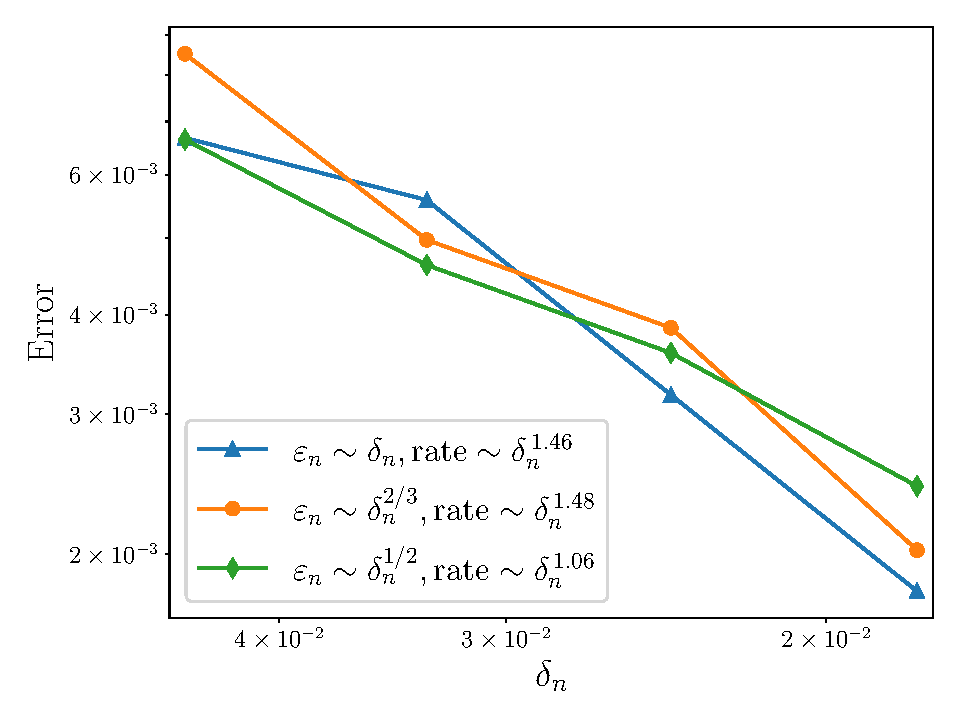
\includegraphics[width=1.02\textwidth]{atelier/aronsson_star_singular_plot}
\end{minipage}%
%
\hfill%
%
\begin{minipage}{.65\textwidth}%
\small
\centering
Ratio convergence rates for\\percolation length scales:
\vskip3pt%
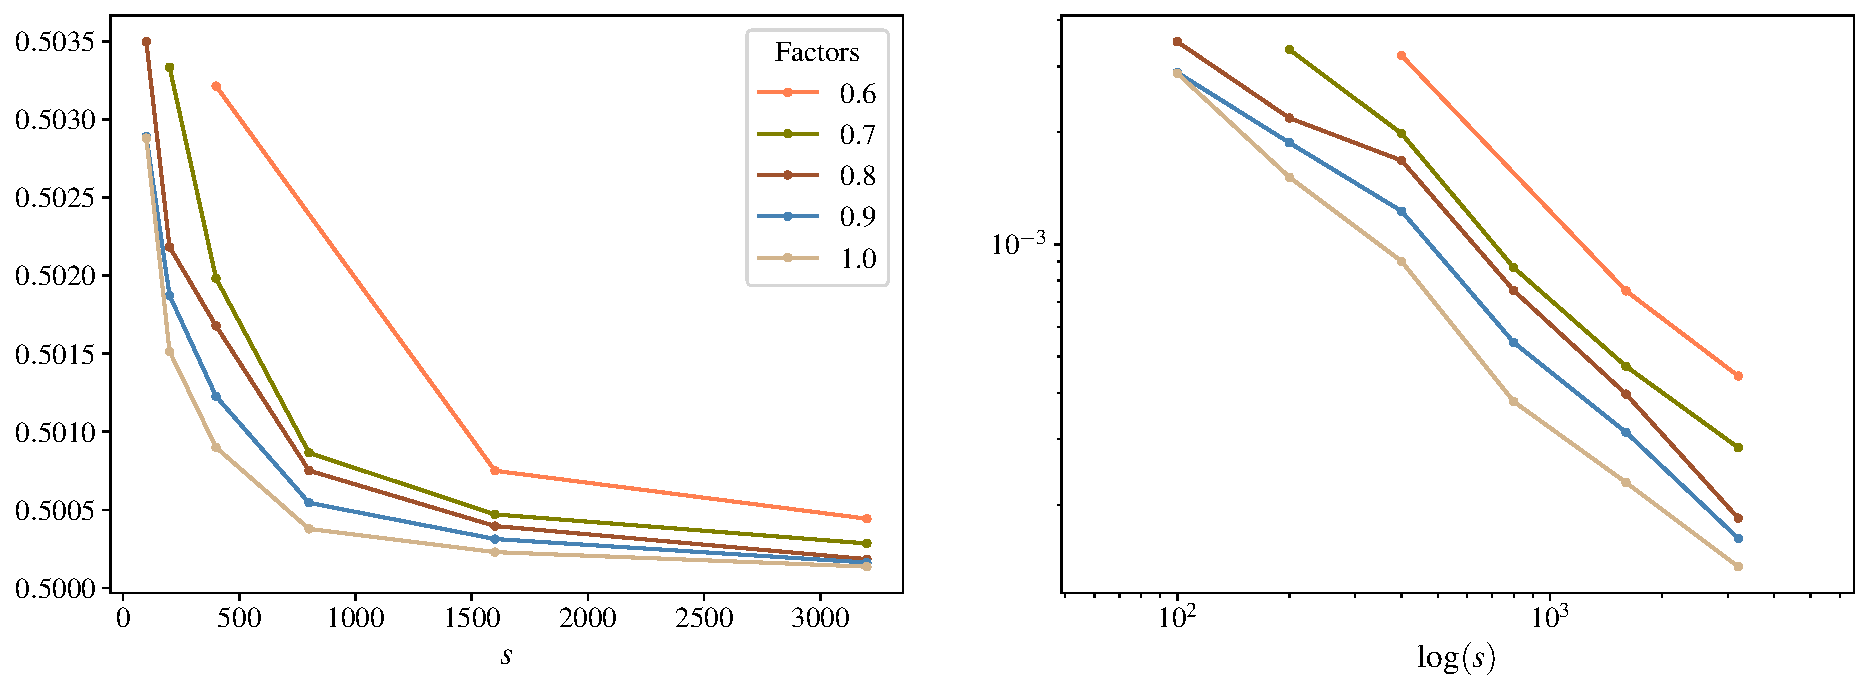
\includegraphics[width=\textwidth]{atelier/ratio_convergence_3d}%
\end{minipage}%
%
{\color{BaseDarkColor}\usebeamerfont{block title} References}
\AtNextBibliography{\tiny}%
\printbibliography[heading=none]


\end{minipage}